\documentclass[crop, tikz]{standalone}

\usepackage[utf8]{inputenc}
% 'crop' is the default for v1.0, before it was 'preview'
%\usetikzlibrary{...}% tikz package already loaded by 'tikz' option

\usetikzlibrary{arrows}
\usetikzlibrary{decorations.markings}

\begin{document}

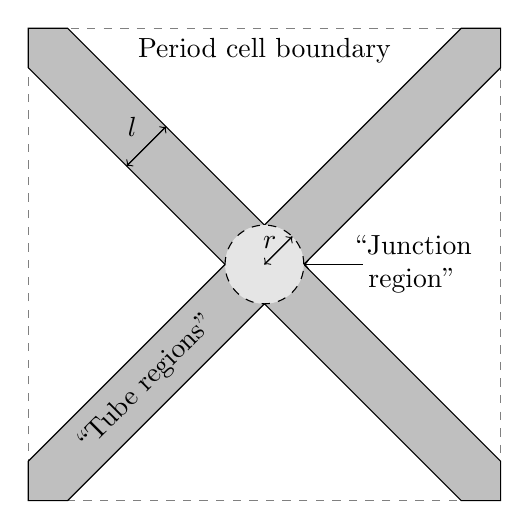
\begin{tikzpicture}

	\draw[dashed, black!50!white] (-3,-3) rectangle (3,3);
	\filldraw[fill=black!25!white, draw=black] (-3,2.5) -- (-0.5,0) -- (-3,-2.5) -- (-3,-3) -- (-2.5,-3) -- (0,-0.5) -- (2.5,-3) -- (3,-3) -- (3,-2.5) -- (0.5,0) -- (3,2.5) -- (3,3) -- (2.5,3) -- (0,0.5) -- (-2.5,3) -- (-3,3) -- cycle;

	%tube width
	\draw[->] (-1.75,1.25) -- (-1.25,1.75);
	\draw[->] (-1.25,1.75) -- (-1.75,1.25);
	\node[anchor=south east] at (-1.5,1.5) {$l$};

	%junction radius
	\draw[black, dashed, fill=black!10!white] (0,0) circle (0.5);
	\draw[->] (0,0) -- (0.5/1.414, 0.5/1.414);
	\draw[->] (0.5/1.414, 0.5/1.414) -- (0,0);
	\node[anchor=south east] at (0.25/1.414 + 0.1, 0.25/1.414 - 0.1) {$r$};

	%tube label
	\node[rotate=45] (TubeLabel) at (-1.5,-1.5) {``Tube  regions"};

	%junction label
	\node[anchor=west, align=center] (JuncLabel) at (1,0) {``Junction \\ region"};
	\draw[->] (1.25,0) -- (0.5,0);

	%period cell boundary
	\node[anchor=north] (BoundLabel) at (0,3) {Period cell boundary};
\end{tikzpicture}

\end{document}